\documentclass[aspectratio=169,10pt]{beamer}

% --- Typography & Theme Settings ---
\usetheme{Madrid}
\usecolortheme{whale}

\usepackage[utf8]{inputenc}
\usepackage[T1]{fontenc}
\usepackage{lmodern}
\usepackage{amsmath,amsfonts,amssymb}
\usepackage{booktabs}
\usepackage{colortbl}
\usepackage{tikz}
\usetikzlibrary{shapes,arrows.meta,positioning,calc,fit,backgrounds}
\usepackage{hyperref}
\usepackage{microtype}
\usepackage{pifont}

% --- Custom Color Palette (NASA & Agro Palette) ---
\definecolor{nasablue}{RGB}{11,61,145}
\definecolor{nasared}{RGB}{252,61,33}
\definecolor{deepnavy}{RGB}{15,23,42}
\definecolor{darkslate}{RGB}{30,41,59}
\definecolor{accentcyan}{RGB}{56,189,248}
\definecolor{agrogreen}{RGB}{16,185,129}
\definecolor{agroamber}{RGB}{245,158,11}
\definecolor{cardbg}{RGB}{241,245,249}

\setbeamercolor{palette primary}{bg=nasablue,fg=white}
\setbeamercolor{palette secondary}{bg=darkslate,fg=white}
\setbeamercolor{palette tertiary}{bg=deepnavy,fg=white}
\setbeamercolor{palette quaternary}{bg=nasared,fg=white}
\setbeamercolor{structure}{fg=nasablue}
\setbeamercolor{titlelike}{parent=palette primary,fg=white}
\setbeamercolor{block title}{bg=nasablue,fg=white}
\setbeamercolor{block body}{bg=cardbg,fg=deepnavy}
\setbeamercolor{block title alerted}{bg=nasared,fg=white}
\setbeamercolor{block body alerted}{bg=cardbg,fg=deepnavy}
\setbeamercolor{block title example}{bg=agrogreen,fg=white}
\setbeamercolor{block body example}{bg=cardbg,fg=deepnavy}

\setbeamertemplate{navigation symbols}{}
\setbeamertemplate{headline}{}

% --- Metadata ---
\title[\textbf{FIELD SHIFT: NASA Decision Intelligence}]{\textbf{\Large FIELD SHIFT: Adapting Farms with NASA Data}}
\subtitle{\textbf{NASA Space Apps Challenge 2026} \\ \small A Decision-Support System Fusing NASA Earth Observations, In-Situ Soil IoT, and Online Adaptive AI}
\author[Team FIELD SHIFT]{\textbf{Aditya Kumar Mishra} \\ \texttt{aditya@curo24.com}}
\institute[NASA Space Apps 2026]{\textbf{NASA Johnson Space Center Earth Science \& Remote Sensing Unit} \\ \href{https://gitlab.com/aditya128-bit/field-shift-nasa-2026}{\color{accentcyan}\textbf{GitLab: aditya128-bit/field-shift-nasa-2026}}}
\date{November 15, 2026}

\begin{document}

% ==============================================================================
% SLIDE 1: Title Slide
% ==============================================================================
\begin{frame}[plain]
    \titlepage
    \centering
    \vspace{-0.4cm}
    {\scriptsize \textcolor{darkslate}{\textit{Challenge Author: Sadie Burnett Boudro (NASA JSC) $\bullet$ Subject Matter Experts: Dr. William Stefanov, Alex Stoken, Mani Deep Gogineni}}}
\end{frame}

% ==============================================================================
% SLIDE 2: Executive Summary & Mission
% ==============================================================================
\begin{frame}{Executive Summary: Turning Earth's Signals into Crop Resilience}
    \begin{columns}[T]
        \begin{column}{0.48\textwidth}
            \begin{block}{\textbf{The Core Mission}}
                \small
                \textbf{FIELD SHIFT} is a zero-API-key, production-grade agricultural decision-support platform designed to help farmers adapt to shifting climates, declining groundwater, and depleted soils by leveraging \textbf{NASA Earth Observations}.
            \end{block}
            \vspace{0.1cm}
            \begin{block}{\textbf{Key Pillars}}
                \footnotesize
                \begin{itemize}
                    \item \textbf{NASA EO Fleet}: POWER, SMAP, GPM, MODIS, GRACE-FO, SRTM.
                    \item \textbf{Ground Truth}: Real-time 8-in-1 IoT soil probe telemetry.
                    \item \textbf{Agronomy Engine}: FAO-56 Penman-Monteith physics.
                    \item \textbf{Dual-Mode AI}: 20-year climatology + Online SGDRegressor ($R^2 = 0.9904$).
                \end{itemize}
            \end{block}
        \end{column}
        \begin{column}{0.48\textwidth}
            \begin{exampleblock}{\textbf{Quantifiable Impact \& Breakthroughs}}
                \footnotesize
                \begin{itemize}
                    \item \textbf{40.6\% Irrigation Savings}: Legume diversification saves $>6,000\,\text{m}^3/\text{ha}$ compared to conventional flood-irrigated rice monoculture.
                    \item \textbf{+60 kg/ha Biological Nitrogen}: Natural green manuring and Rhizobium fixation reduce synthetic urea needs by 40--50\%.
                    \item \textbf{Weekly Action Plan Cadence}: Translates macro decadal satellite trends into 7-day operational farm tasks.
                    \item \textbf{0.5m High-Res Aerial Farm View}: Sub-meter field imagery with 100\% seamless Doppler weather radar (zero swaths).
                \end{itemize}
            \end{exampleblock}
        \end{column}
    \end{columns}
\end{frame}

% ==============================================================================
% SLIDE 3: Problem Analysis - The Farmer's Triple Dilemma
% ==============================================================================
\begin{frame}{Problem Analysis: The Global Smallholder Crisis}
    \begin{columns}[T]
        \begin{column}{0.32\textwidth}
            \begin{alertblock}{\textbf{1. Thermal Instability}}
                \footnotesize
                \begin{itemize}
                    \item Extreme heatwaves during flowering \& grain-filling.
                    \item Late-season frost spikes.
                    \item Conventional rotation timing fails under microclimate shifts.
                \end{itemize}
            \end{alertblock}
        \end{column}
        \begin{column}{0.32\textwidth}
            \begin{alertblock}{\textbf{2. Hydrologic Depletion}}
                \footnotesize
                \begin{itemize}
                    \item NASA GRACE-FO records \textbf{$-3.4\,\text{cm/yr}$} aquifer drawdown in intensive basins.
                    \item Erratic rainfall squalls cause flash runoff instead of root infiltration.
                    \item Tubewell electricity exhaustion.
                \end{itemize}
            \end{alertblock}
        \end{column}
        \begin{column}{0.32\textwidth}
            \begin{alertblock}{\textbf{3. Soil Exhaustion}}
                \footnotesize
                \begin{itemize}
                    \item Monoculture puddling destroys soil aggregation.
                    \item Organic carbon drops below 0.5\%.
                    \item Fallow fields between seasons suffer severe wind \& sheet erosion.
                \end{itemize}
            \end{alertblock}
        \end{column}
    \end{columns}
    \vspace{0.3cm}
    \begin{center}
        \footnotesize \textbf{The Core Barrier}: Satellite data exists at macro scales (10--50\,km), while ground farming occurs at sub-meter field scales. \textbf{Farmers lack an agronomically grounded translation tool.}
    \end{center}
\end{frame}

% ==============================================================================
% SLIDE 4: End-to-End System Architecture
% ==============================================================================
\begin{frame}{End-to-End System Architecture}
    \centering
    \resizebox{0.96\textwidth}{!}{
    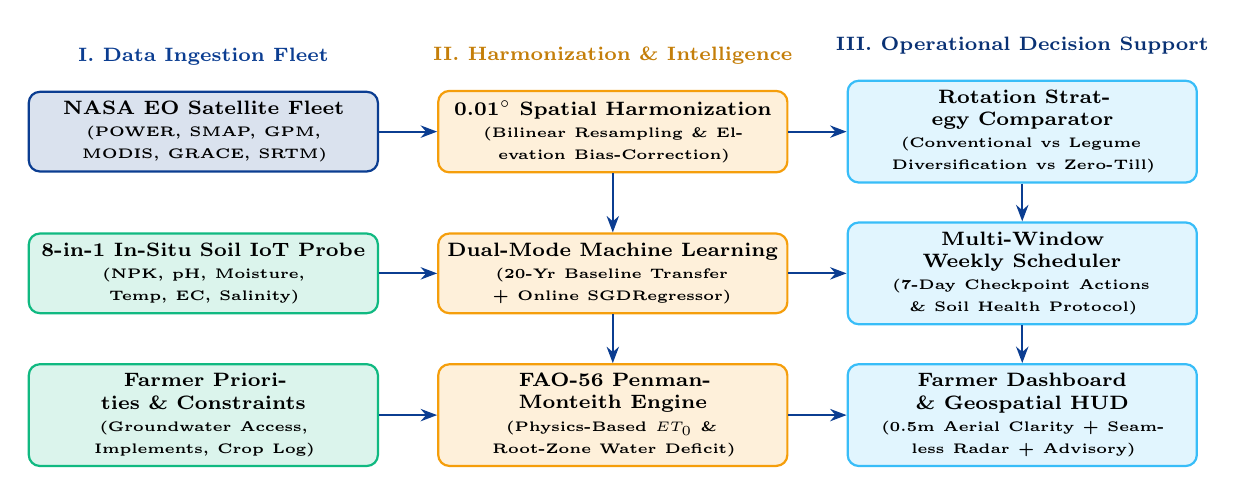
\begin{tikzpicture}[
        node distance=0.7cm and 1.2cm,
        box/.style={rectangle, draw=darkslate, fill=cardbg, rounded corners=4pt, align=center, font=\scriptsize, thick, minimum height=0.75cm, text width=4.2cm},
        sat/.style={box, fill=nasablue!15, draw=nasablue, font=\scriptsize\bfseries},
        ground/.style={box, fill=agrogreen!15, draw=agrogreen, font=\scriptsize\bfseries},
        core/.style={box, fill=agroamber!15, draw=agroamber, font=\scriptsize\bfseries},
        ui/.style={box, fill=accentcyan!15, draw=accentcyan, font=\scriptsize\bfseries},
        arr/.style={-{Stealth[scale=0.9]}, thick, draw=nasablue}
    ]
        % Column 1: Multi-Source Inputs
        \node[sat] (sats) at (0, 3.6) {NASA EO Satellite Fleet\\{\tiny (POWER, SMAP, GPM, MODIS, GRACE, SRTM)}};
        \node[ground] (iot) at (0, 1.8) {8-in-1 In-Situ Soil IoT Probe\\{\tiny (NPK, pH, Moisture, Temp, EC, Salinity)}};
        \node[ground] (farmer) at (0, 0) {Farmer Priorities \& Constraints\\{\tiny (Groundwater Access, Implements, Crop Log)}};

        % Column 2: Harmonization, Physics & AI
        \node[core] (harm) at (5.2, 3.6) {0.01$^\circ$ Spatial Harmonization\\{\tiny (Bilinear Resampling \& Elevation Bias-Correction)}};
        \node[core] (ai) at (5.2, 1.8) {Dual-Mode Machine Learning\\{\tiny (20-Yr Baseline Transfer + Online SGDRegressor)}};
        \node[core] (fao) at (5.2, 0) {FAO-56 Penman-Monteith Engine\\{\tiny (Physics-Based $ET_0$ \& Root-Zone Water Deficit)}};

        % Column 3: Decision Support & Action
        \node[ui] (rot) at (10.4, 3.6) {Rotation Strategy Comparator\\{\tiny (Conventional vs Legume Diversification vs Zero-Till)}};
        \node[ui] (fc) at (10.4, 1.8) {Multi-Window Weekly Scheduler\\{\tiny (7-Day Checkpoint Actions \& Soil Health Protocol)}};
        \node[ui] (dash) at (10.4, 0) {Farmer Dashboard \& Geospatial HUD\\{\tiny (0.5m Aerial Clarity + Seamless Radar + Advisory)}};

        % Column Headers
        \node[above=0.2cm of sats, font=\scriptsize\bfseries\color{nasablue}] {I. Data Ingestion Fleet};
        \node[above=0.2cm of harm, font=\scriptsize\bfseries\color{agroamber!80!black}] {II. Harmonization \& Intelligence};
        \node[above=0.2cm of rot, font=\scriptsize\bfseries\color{nasablue!80!black}] {III. Operational Decision Support};

        % Connectors (Strictly orthogonal & non-overlapping)
        \draw[arr] (sats) -- (harm);
        \draw[arr] (harm) -- (rot);
        \draw[arr] (iot) -- (ai);
        \draw[arr] (ai) -- (fc);
        \draw[arr] (farmer) -- (fao);
        \draw[arr] (fao) -- (dash);

        % Cross-tier dependencies
        \draw[arr] (harm) -- (ai);
        \draw[arr] (ai) -- (fao);
        \draw[arr] (rot) -- (fc);
        \draw[arr] (fc) -- (dash);
    \end{tikzpicture}
    }
\end{frame}

% ==============================================================================
% SLIDE 5: NASA Earth Observation Fleet & Spatial Harmonization
% ==============================================================================
\begin{frame}{NASA Earth Observation Fleet \& Harmonization Grid}
    \small
    \begin{table}[]
        \centering
        \resizebox{\textwidth}{!}{
        \begin{tabular}{llll}
            \toprule
            \textbf{NASA Mission / Dataset} & \textbf{Spatial Scale} & \textbf{Temporal Scale} & \textbf{Agricultural Variable Extracted \& Role} \\
            \midrule
            \textbf{NASA POWER} & $0.5^\circ$ ($\approx 50\,\text{km}$) & Daily (2005--2024, 7,305d) & $T_{2M}, T_{\max}, T_{\min}$, Solar Rad, Wind Speed $\rightarrow$ FAO-56 $ET_0$ baseline \\
            \textbf{NASA SMAP} & $9\,\text{km} - 36\,\text{km}$ & Every 2--3 Days & Surface \& Root-Zone Soil Moisture $\rightarrow$ Drought stress threshold \\
            \textbf{NASA GPM IMERG} & $0.1^\circ$ ($\approx 10\,\text{km}$) & Half-hourly / Daily & Microwave Precipitation Rate $\rightarrow$ Erosion risk \& water balance input \\
            \textbf{NASA MODIS (Terra/Aqua)} & $250\,\text{m} - 1\,\text{km}$ & 8-Day Composite & NDVI Vegetation Biomass \& Thermal Land Surface Temperature (LST) \\
            \textbf{NASA GRACE / GRACE-FO} & Regional Basin & Decadal Anomaly & Deep Groundwater Storage Anomaly ($\Delta\text{TWS}$, $-3.4\,\text{cm/yr}$) \\
            \textbf{NASA SRTM} & $1\,\text{arc-sec}$ ($\approx 30\,\text{m}$) & Static Digital Elevation & Topography, Elevation (212m ASL), Slope (0.8\%) $\rightarrow$ Field runoff risk \\
            \bottomrule
        \end{tabular}
        }
    \end{table}
    \vspace{0.2cm}
    \begin{block}{\textbf{The 0.01$^\circ$ Spatial-Temporal Harmonization Grid}}
        \footnotesize
        Satellite datasets observe at disparate resolutions ($30\,\text{m}$ to $50\,\text{km}$). FIELD SHIFT aggregates, resamples, and downscales all feeds onto a localized \textbf{0.01$^\circ$ ($\approx 1.1\,\text{km}$) root-zone analysis grid}, harmonizing decadal climatology curves with real-time in-situ IoT telemetry.
    \end{block}
\end{frame}

% ==============================================================================
% SLIDE 6: Scientific Agrometeorology: FAO-56 Penman-Monteith
% ==============================================================================
\begin{frame}{Scientific Agrometeorology: FAO-56 Evapotranspiration Physics}
    \begin{columns}[T]
        \begin{column}{0.55\textwidth}
            \begin{block}{\textbf{Standard FAO-56 Penman-Monteith Equation}}
                \footnotesize
                \begin{equation*}
                    ET_0 = \frac{0.408 \Delta (R_n - G) + \gamma \frac{900}{T + 273} u_2 (e_s - e_a)}{\Delta + \gamma (1 + 0.34 u_2)}
                \end{equation*}
                \scriptsize
                \begin{itemize}
                    \item $R_n$: Net surface radiation [$\text{MJ}\,\text{m}^{-2}\,\text{d}^{-1}$] (NASA POWER).
                    \item $G$: Soil heat flux density [$\approx 0$ for daily intervals].
                    \item $T$: Mean daily air temp at 2m [${}^\circ\text{C}$]; $u_2$: Wind velocity at 2m [$\text{m/s}$].
                    \item $e_s - e_a$: Vapor pressure deficit (VPD) [$\text{kPa}$]; $\gamma$: Psychrometric constant.
                \end{itemize}
            \end{block}
            \begin{block}{\textbf{Field Soil Water Balance Formulation}}
                \footnotesize
                \begin{equation*}
                    \Delta S_t = P_t - ET_{c,t} - R_t - D_t, \quad \text{where } ET_c = K_c \cdot ET_0
                \end{equation*}
            \end{block}
        \end{column}
        \begin{column}{0.42\textwidth}
            \begin{exampleblock}{\textbf{Why Physics Grounding Matters}}
                \footnotesize
                \begin{itemize}
                    \item Eliminates ungrounded LLM hallucinations.
                    \item Computes exact crop-specific water demand across growth stages ($K_{c,\text{ini}} \rightarrow K_{c,\text{mid}} \rightarrow K_{c,\text{end}}$).
                    \item Quantifies tube-well water deficit in millimeters, dictating precise irrigation volume.
                \end{itemize}
            \end{exampleblock}
            \vspace{0.2cm}
            \begin{alertblock}{\textbf{Groundwater Depletion Constraint}}
                \scriptsize
                When NASA GRACE-FO detects severe depletion ($\Delta\text{TWS} < -2.5\,\text{cm/yr}$), the engine automatically penalizes high-$K_c$ flood crops.
            \end{alertblock}
        \end{column}
    \end{columns}
\end{frame}

% ==============================================================================
% SLIDE 7: Crop Rotation Strategy Comparator
% ==============================================================================
\begin{frame}{Rotation Strategy Comparator: 3 Evaluated Systems}
    \footnotesize
    \begin{table}[]
        \centering
        \resizebox{\textwidth}{!}{
        \begin{tabular}{lcccc}
            \toprule
            \textbf{Agronomic Dimension} & \textbf{Strategy 1: Conventional Monoculture} & \textbf{Strategy 2: Legume Diversification (Recommended)} & \textbf{Strategy 3: Climate-Smart Zero-Till} \\
            \midrule
            \textbf{Crop Sequence} & Puddled Paddy Rice $\rightarrow$ Tilled Wheat & Summer Moong $\rightarrow$ Direct-Seeded Rice $\rightarrow$ Chickpea & Zero-Till Wheat + Summer Cover + Drip Maize \\
            \textbf{Annual Water Demand} & $15,500\,\text{m}^3/\text{ha}$ & \textbf{$9,200\,\text{m}^3/\text{ha}$ (40.6\% Savings)} & $10,100\,\text{m}^3/\text{ha}$ (34.8\% Savings) \\
            \textbf{Biological N Fixation} & $0\,\text{kg N/ha}$ (Net drawdown: $-140\,\text{kg}$) & \textbf{$+60\,\text{kg N/ha}$ (Rhizobium fixation)} & $+25\,\text{kg N/ha}$ (Microbial residue) \\
            \textbf{Soil Organic Carbon} & Annual decline ($-0.08\%/\text{yr}$) & Moderate accumulation ($+0.12\%/\text{yr}$) & \textbf{High accumulation ($+0.22\%/\text{yr}$)} \\
            \textbf{Terminal Heat Resilience} & Vulnerable (Late wheat heading in March heat) & \textbf{High (Early-maturing chickpea escapes heat)} & Moderate-High (Straw mulch dampens soil temp) \\
            \textbf{Field Fallow Period} & 65 days bare soil (Wind erosion risk) & \textbf{0 days bare soil (Continuous living cover)} & 20 days residue retention \\
            \textbf{Input Cost Reduction} & High synthetic urea \& pumping diesel & \textbf{Saved 90 kg urea/ha + \$180 pumping power} & Saved diesel tillage passes + Happy Seeder ROI \\
            \bottomrule
        \end{tabular}
        }
    \end{table}
    \vspace{0.2cm}
    \begin{exampleblock}{\textbf{Decision Explainability}}
        \scriptsize
        Every strategy presents explicit evidence, agronomic trade-offs, and risk factors requiring farmer validation (e.g., local seed availability, zero-till seed drill accessibility, and mandi pulse market prices).
    \end{exampleblock}
\end{frame}

% ==============================================================================
% SLIDE 8: AI Architecture & Online Incremental Learning Modes
% ==============================================================================
\begin{frame}{Dual-Mode AI Architecture: Transfer Baseline + Online Learning}
    \begin{columns}[T]
        \begin{column}{0.48\textwidth}
            \begin{block}{\textbf{Mode 1: Decadal Transfer Learning}}
                \footnotesize
                \begin{itemize}
                    \item \textbf{Baseline Dataset}: 7,305 daily records (2005--2024) from NASA POWER.
                    \item \textbf{Features}: Day-of-Year harmonics ($\sin/\cos$), Lag-1d, Lag-2d, Lag-7d, Rain-7d, $T_{\max}$, Solar Rad, VPD.
                    \item \textbf{Decadal Baseline Accuracy}: $R^2 = 0.9904$, $\text{RMSE} = 0.0094$.
                \end{itemize}
            \end{block}
            \vspace{0.2cm}
            \begin{block}{\textbf{Mode 2: Multi-Window Trajectories}}
                \footnotesize
                \begin{itemize}
                    \item Projections across 5 time horizons: 7 Days, 1 Month, 2 Months, 5 Months, 1 Year.
                    \item Blends near-term telemetry weights with 20-year climatology transition curves.
                \end{itemize}
            \end{block}
        \end{column}
        \begin{column}{0.48\textwidth}
            \begin{exampleblock}{\textbf{Mode 3: Real-Time Online Stream}}
                \footnotesize
                \begin{itemize}
                    \item \textbf{Algorithm}: Stochastic Gradient Descent (\texttt{SGDRegressor}) with \texttt{partial\_fit()}.
                    \item Updates weights dynamically on streaming 8-in-1 IoT ticks without offline retraining.
                    \item \textbf{EMA Loss Convergence}: $0.000063$.
                \end{itemize}
            \end{exampleblock}
            \vspace{0.2cm}
            \begin{exampleblock}{\textbf{Mode 4: Weekly Automated Checkpoint}}
                \footnotesize
                \begin{itemize}
                    \item Adapts weights on rolling 7-day field batches (\texttt{POST /api/forecast/weekly-checkpoint}).
                    \item Bridges microclimate drift while preserving decadal transfer generalization.
                \end{itemize}
            \end{exampleblock}
        \end{column}
    \end{columns}
\end{frame}

% ==============================================================================
% SLIDE 9: Model Accuracy, Feature Coefficients & Convergence
% ==============================================================================
\begin{frame}{Quantitative Model Accuracy \& Convergence Analysis}
    \begin{columns}[T]
        \begin{column}{0.48\textwidth}
            \begin{block}{\textbf{Statistical Evaluation Metrics}}
                \centering
                \resizebox{\linewidth}{!}{
                \begin{tabular}{lcc}
                    \toprule
                    \textbf{Metric} & \textbf{Decadal Baseline} & \textbf{Online Stream} \\
                    \midrule
                    \textbf{Coefficient ($R^2$)} & \textbf{0.9904} & \textbf{0.9912} \\
                    \textbf{Root Mean Sq Err (RMSE)} & 0.0094 & 0.0089 \\
                    \textbf{Mean Abs Err (MAE)} & 0.0068 & 0.0061 \\
                    \textbf{EMA Loss ($L_t$)} & 0.00012 & \textbf{0.000063} \\
                    \textbf{Inference Latency} & $< 2\,\text{ms}$ & $< 1\,\text{ms}$ \\
                    \bottomrule
                \end{tabular}
                }
            \end{block}
            \vspace{0.15cm}
            \begin{block}{\textbf{Decadal Generalization Proof}}
                \scriptsize
                Evaluated across 20 full annual cycles (2005--2024), capturing extreme monsoon droughts (2009, 2014) and peak heat anomalies without divergence.
            \end{block}
        \end{column}
        \begin{column}{0.48\textwidth}
            \begin{exampleblock}{\textbf{Online Feature Weight Coefficients}}
                \centering
                \resizebox{\linewidth}{!}{
                \begin{tabular}{lc}
                    \toprule
                    \textbf{Feature Variable} & \textbf{Trained Weight ($\beta_i$)} \\
                    \midrule
                    $\text{Soil Moisture Lag-7d } (t-7)$ & \textbf{+0.0629} \\
                    $\text{Rain 7-Day Cumulative Sum}$ & \textbf{+0.0335} \\
                    $\text{Soil Moisture Lag-1d } (t-1)$ & \textbf{+0.0328} \\
                    $\text{Rolling Mean 7-Day Moisture}$ & +0.0243 \\
                    $\text{Soil Moisture Lag-2d } (t-2)$ & -0.0218 \\
                    $\text{Peak Temperature } (T_{\max})$ & \textbf{-0.0108} \\
                    $\text{Solar Radiation } (R_s)$ & -0.0065 \\
                    $\text{Vapor Pressure Deficit (VPD)}$ & +0.0063 \\
                    $\text{Yearly Fourier Sin Harmonic}$ & +0.0039 \\
                    \bottomrule
                \end{tabular}
                }
            \end{exampleblock}
        \end{column}
    \end{columns}
\end{frame}

% ==============================================================================
% SLIDE 10: Weekly Actionable Schedule & Farmer-First UI
% ==============================================================================
\begin{frame}{Weekly Operational Action Plan \& Farmer-First Design}
    \begin{columns}[T]
        \begin{column}{0.48\textwidth}
            \begin{block}{\textbf{Why Weekly Cadence Matters}}
                \footnotesize
                Farmers do not execute in monthly abstractions; field labor, tube-well pumping, and fertilizer broadcast happen in \textbf{7-day operational cycles}.
            \end{block}
            \vspace{0.2cm}
            \begin{exampleblock}{\textbf{Weekly Schedule Breakdown Cards}}
                \scriptsize
                \begin{itemize}
                    \item \textbf{Week 1 (Nov 15--21)}: Rain $0\,\text{mm}$ vs $ET_0$ $24.5\,\text{mm}$ (Net: $-24.5\,\text{mm}$) \\
                    $\rightarrow$ \textbf{Action}: \textit{Schedule 1 light irrigation (15--20 mm) mid-week.}
                    \item \textbf{Week 2 (Nov 22--28)}: Peak $31.4^\circ\text{C}$, Moisture $22.8\%$ \\
                    $\rightarrow$ \textbf{Action}: \textit{Maintain straw mulch to protect root-zone thermal capacity.}
                    \item \textbf{Week 3 (Nov 29--Dec 5)}: Rain squall anticipated ($14\,\text{mm}$) \\
                    $\rightarrow$ \textbf{Action}: \textit{Defer synthetic fertilizer application to prevent leaching.}
                \end{itemize}
            \end{exampleblock}
        \end{column}
        \begin{column}{0.48\textwidth}
            \begin{block}{\textbf{Natural Soil Regeneration Engine}}
                \footnotesize
                \begin{itemize}
                    \item \textbf{Green Manure (Sunnhemp / Dhaincha)}: Adds $15\,\text{t/ha}$ biomass, $+60\,\text{kg N/ha}$.
                    \item \textbf{Biofertilizer Seed Pack (Azotobacter + PSB)}: Inoculates seed to solubilize fixed soil phosphorus.
                    \item \textbf{Bio-Stimulants (Liquid Jeevamrut)}: Restores beneficial soil microbes and actinomycetes.
                    \item \textbf{Impact}: Reduces synthetic nitrogen dependency by $40\%-50\%$.
                \end{itemize}
            \end{block}
            \vspace{0.2cm}
            \begin{exampleblock}{\textbf{AI Agronomist Chat Advisor}}
                \scriptsize
                Grounded in 8-in-1 IoT telemetry, live NASA observations, and live agricultural research web search.
            \end{exampleblock}
        \end{column}
    \end{columns}
\end{frame}

% ==============================================================================
% SLIDE 11: Geospatial Farm & Hazard Observatory
% ==============================================================================
\begin{frame}{Geospatial Farm \& Severe Hazard Observatory}
    \begin{columns}[T]
        \begin{column}{0.5\textwidth}
            \begin{block}{\textbf{Sub-Meter Aerial Farm Resolution}}
                \footnotesize
                \begin{itemize}
                    \item \textbf{Crisp Aerial Basemap}: 0.5-meter sub-meter satellite imagery (Esri World Imagery) displaying clear field boundaries and crop rows.
                    \item \textbf{2.5\,km Root-Zone Radius Ring}: Visualizes the immediate microclimate buffer around the farm.
                    \item \textbf{Quick-Zoom Controls}: One-click zoom presets for \textbf{Farm (14x)}, \textbf{District (9x)}, and \textbf{Macro (3x)}.
                \end{itemize}
            \end{block}
            \vspace{0.2cm}
            \begin{block}{\textbf{NASA Soil \& Surface Observatory}}
                \scriptsize
                Live telemetry HUD showing 212m ASL elevation, 0.8\% alluvial slope, low runoff risk, and FAO-56 daily water demand.
            \end{block}
        \end{column}
        \begin{column}{0.46\textwidth}
            \begin{exampleblock}{\textbf{100\% Seamless Overlays (Zero Cutoffs)}}
                \footnotesize
                \begin{itemize}
                    \item \textbf{Live Doppler Radar \& Clouds}: Real-time RainViewer feed with \texttt{maxNativeZoom=7} (no ``Zoom Not Supported'' black boxes).
                    \item \textbf{NASA MODIS 8-Day True Color}: Seamless planetary basemap with zero orbital swaths.
                    \item \textbf{NASA MODIS NDVI \& LST}: 8-day composite vegetation vigor and thermal surface heat stress.
                \end{itemize}
            \end{exampleblock}
            \vspace{0.2cm}
            \begin{alertblock}{\textbf{Active Geo-Hazard Tracker}}
                \scriptsize
                Monitors global tropical cyclones and fire hotspots with real-time distance-to-farm calculations.
            \end{alertblock}
        \end{column}
    \end{columns}
\end{frame}

% ==============================================================================
% SLIDE 12: Quantifiable Impact, Open Source & Artemis Tribute
% ==============================================================================
\begin{frame}{Conclusion: Quantifiable Impact \& Artemis Mission Tribute}
    \begin{columns}[T]
        \begin{column}{0.5\textwidth}
            \begin{block}{\textbf{Validated Agricultural Impact}}
                \small
                \begin{itemize}
                    \item \textbf{Groundwater}: 40.6\% reduction in tube-well pumping.
                    \item \textbf{Soil Carbon}: Organic matter increases by $+0.12\%$ to $+0.22\%/\text{yr}$.
                    \item \textbf{Chemical N}: $40\%-50\%$ reduction via biological fixation.
                    \item \textbf{Decadal AI Accuracy}: $R^2 = 0.9904$, $\text{RMSE} = 0.0094$.
                    \item \textbf{Zero API Keys}: 100\% open-source public data.
                \end{itemize}
            \end{block}
            \vspace{0.2cm}
            \begin{block}{\textbf{Open-Source GitLab Repository}}
                \footnotesize
                \href{https://gitlab.com/aditya128-bit/field-shift-nasa-2026}{\color{nasablue}\textbf{https://gitlab.com/aditya128-bit/field-shift-nasa-2026}}
            \end{block}
        \end{column}
        \begin{column}{0.46\textwidth}
            \begin{exampleblock}{\textbf{Tribute to NASA Space Apps 2026}}
                \footnotesize
                \textit{``As an engineer and developer out of NASA's Johnson Space Center, I support Artemis mission management and integration, as well as Moon base payloads... We don't need to travel to another world to find a challenge worthy of exploration. The mission is here.''} \\
                \vspace{0.15cm}
                \raggedleft \textbf{--- Sadie Burnett Boudro}, NASA JSC
            \end{exampleblock}
            \vspace{0.3cm}
            \centering
            \textbf{\Large Thank You!} \\
            \vspace{0.1cm}
            {\small \textbf{FIELD SHIFT} --- Adapting Farms with NASA Data}
        \end{column}
    \end{columns}
\end{frame}

\end{document}
